\documentclass{article}
\usepackage[utf8]{inputenc}

\title{Programming Languages}
\author{scifi6546 }
\date{March 2020}


\usepackage{listings}
\usepackage{color}
\usepackage{graphicx}
\graphicspath{ {./} }
\definecolor{dkgreen}{rgb}{0,0.6,0}
\definecolor{gray}{rgb}{0.5,0.5,0.5}
\definecolor{mauve}{rgb}{0.58,0,0.82}

\lstset{frame=tb,
  language=Java,
  aboveskip=3mm,
  belowskip=3mm,
  showstringspaces=false,
  columns=flexible,
  basicstyle={\small\ttfamily},
  numbers=none,
  numberstyle=\tiny\color{gray},
  keywordstyle=\color{blue},
  commentstyle=\color{dkgreen},
  stringstyle=\color{mauve},
  breaklines=true,
  breakatwhitespace=true,
  tabsize=3
}
\begin{document}

\maketitle

\section{Introduction to Open Shading Language}
The purpose of Open Shading Language (OSL) is to create programs that are used by a raytacing rendering engines to draw scenes. Open Shading Language is used in many rendering engines such as blender's cycles engine and V-Ray. OSL has a different focus then a traditional shading languages such as glsl because OSL outputs materials rather then directly calculating RGB values. The rendering engine then uses the generated materials to calculate the trajectory of rays of light in order to render the correct color for the object. 
\section{Features}
OSL has a c like syntax.
\section{Execution}
OSL is ececuted with a SIMD architecture. Each shader outputs a closure that can be run in parallel. The rendering engine then executes the closures to calculate the trajectory of rays of light when they hit a object with the current shader.  Rendering is commonly accelerated using General Purpose Graphics Processing Units (GPGPU). For example Blender uses OpenCL and CUDA to accelerate rendering \cite{blender_gpu}. The output of shader programs are used as input of other programs. In blender the shaders can be combined using a GUI node based system as shown in the figure below. \newline
INSERT BLENDER FIGURES HERE
\newline
The GUI system is then used by artists to generate the desired graphics, such as a wood material for a floor.
\section{Example Code}
All of the below examples are shaders that are placed onto a sphere with a single sun light and no global illumination. The code sample below is a simple white diffuse material.
\begin{lstlisting}
shader simple_material(
  output closure color BSDF = diffuse(N)){
    BSDF = diffuse(N);
  }
}
\end{lstlisting}
\begin{figure}
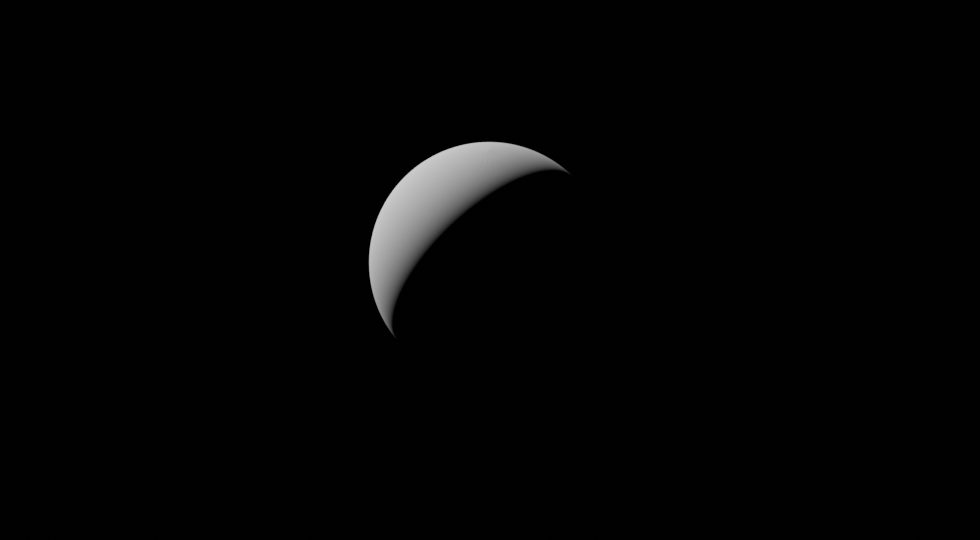
\includegraphics[width=10cm]{hello_sphere.png}
\centering
\end{figure}

\begin{thebibliography}{9}

\bibitem{blender_gpu}
  Blender Manual,
  https://docs.blender.org/manual/en/latest/render/cycles/gpu\_rendering.html,

\end{thebibliography}
\end{document}